\documentclass[a4paper,10pt]{article}

\usepackage[utf8]{inputenc} % pour les accents
\usepackage[T1]{fontenc} % caracteres francais
\usepackage{geometry} %les marges
\usepackage[french]{babel} %langue principale
\usepackage[dvips]{graphicx}
\geometry{ hmargin=2cm, vmargin=2cm }

\pagestyle{empty} %pas de numerotation de page

%
% Debut du document
%
\begin{document}

\section*{FICHE DE VALIDATION DU LOGICIEL MASCARET V7P0}

\subsection*{Validation du noyau transcritique}

\subsection*{\emph{Etude réelle d'onde de submersion}}

\subsection*{Numéro du cas test : 23}

\subsection*{Auteur : Fabrice ZAOUI}



\vspace{1cm}

\subsection*{Description}

Ce cas test consiste en une simulation d'onde de submersion dans une vallée réelle. Le barrage principal est supposé rompre instantanément. La vallée comporte $3$ affluents et $3$ barrages situés à l'aval du barrage principal (voir la figure~\ref{fig1}).

\subsection*{Données géométriques}

La vallée principale a une longueur de $100\ km$. Les trois affluents modélisés ont des longueurs respectives de $6.5\ km$, $4.5\ km$ et $3\ km$. 

La forme de la vallée principale et des affluents est représentée à partir des profils en travers déterminés sur les cartes IGN au $1/25000$ ème et des relevés effectués par le service du Nivellement Général de la France. La densité moyenne des profils est de $2$ profils par $km$.

\subsection*{Données physiques}

\begin{itemize}
 \item Conditions aux limites :
 \begin{itemize}
  \item Débit imposé à l'amont de chaque bief;
  \item Sortie libre à l'aval du bief principal. 
 \end{itemize}
 \item Frottement : coefficient de Strickler constant égal à 30.
 \item Conditions initiales : 
 \begin{itemize}
  \item Fond sec hormis dans les retenues;
  \item Débit nul. 
 \end{itemize}
 \item Barrage principal : rupture instantanée à la cote ``\emph{de plus hautes eaux}'' égale à $418\ m (NGF)$;
 \item Description des ouvrages :


\begin{center}
  \begin{footnotesize}
   \label{tab1}
   \begin{tabular}{|c|c|c|c|c|c|}
   \hline
   & Positionnement (km) & Déversement (m NGF) & Retenue (m NGF) & Coef. débit & Comportement \\
   \hline
   Barrage 1 & 26 &  344 & 343 & 0.38 & casse instantanément \\
   Barrage 2 & 56.3 & 264 & 263 & 0.38 & résiste \\
   Barrage 3 & 64.2 & 195.04 & 194.5 & 0.38 & résiste \\
   \hline
   \end{tabular}
  \end{footnotesize}
\end{center}

\vspace{0.5cm}

 \item Affluents : ils sont situés aux PK $9.9$, $36.2$ et $63.06$ de la vallée principale. La figure~\ref{fig2} présente leur modélisation. 
\end{itemize}

\subsection*{Données numériques}

\begin{itemize}
 \item Pas de temps variable fixé par un nombre de Courant égal à $0.8$;
 \item Durée de la simulation : $9800\ s$;
 \item Modélisation implicite du frottement;
 \item Pas de planimétrage : $1.5\ m$;
 \item Maillage régulier avec un pas de $100\ m$.
\end{itemize}


\subsection*{Résultats}

Sur les figures~\ref{fig3} et \ref{fig4}, sont représentées d'une part la ligne d'eau maximale obtenue au cours de la simulation et les lignes d'eau à différents instants d'autre part. Le premier barrage situé à l'aval du barrage principal casse instantanément et les deux autres résistent tout le long du calcul.

Sur la figure~\ref{fig5}, les débits maximaux obtenus avec Mascaret $v7.0$ sont comparés avec les résultats d'une version plus ancienne du code. La différence constatée (décalage) s'explique par le pas de temps variable calculé qui n'est pas le même entre les deux codes. A la fin de chaque essai, la période de temps simulée n'est donc pas la même. Par ailleurs, il a été vérifié qu'en imposant un même pas de temps fixe pour les deux codes (satisfaisant le CFL de $0.8$), les résultats étaient bien identiques.

Sur la figure~\ref{fig6}, on s'intéresse à la variable débit et plus particulièrement à ses variations au niveau des singularités. Au passage du barrage $2$, on a tracé le débit à l'amont et à l'aval. On remarque qu'il n'y a aucun effet d'écrêtement, ce qui est tout à fait normal puisque la retenue est pleine.

Les évolutions temporelles de débit dans le bief principal à l'amont et à l'aval de l'affluent et dans l'affluent sont données sur la figure~\ref{fig7}. On remarque la montée de débit dans l'affluent au début de la simulation et ensuite la vidange qui crée un second pic de débit dans le bief principal.

Pour ce calcul, l'erreur relative sur la conservativité est de $4.6\ 10^{-2}$.

%\newpage

\begin{figure}
 \begin{center}
  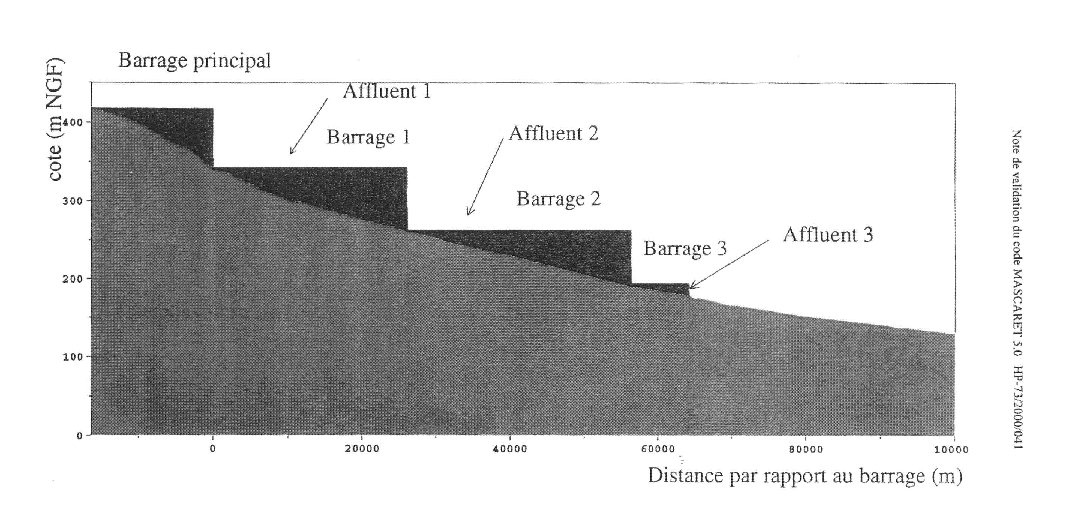
\includegraphics[angle=0,width=17cm]{cond_ini.eps}
  \caption{Conditions initiales}
  \label{fig1}
 \end{center}
\end{figure}

\begin{figure}
 \begin{center}
  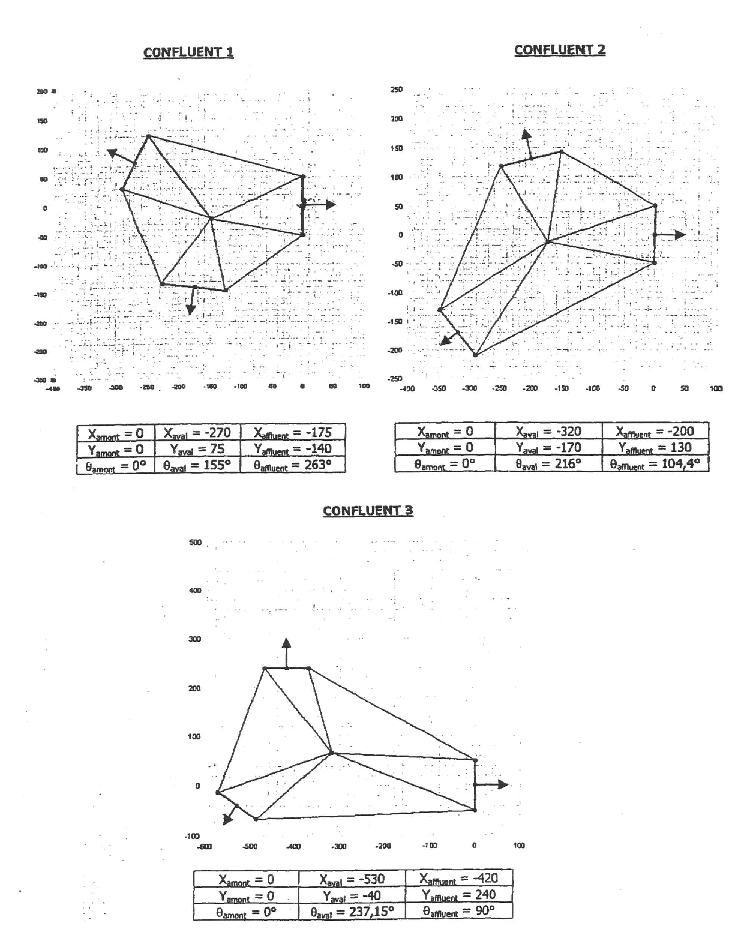
\includegraphics[angle=0,width=17cm]{geom_conflu.eps}
  \caption{Géométrie des confluents}
  \label{fig2}
 \end{center}
\end{figure}

\begin{figure}
 \begin{center}
  \includegraphics[angle=270,width=15cm]{cote_max.eps}
  \caption{Cotes maximales au cours de la simulation}
  \label{fig3}
 \end{center}
\end{figure}

\begin{figure}
 \begin{center}
  \includegraphics[angle=270,width=15cm]{evol_cotes.eps}
  \caption{Evolution des cotes}
  \label{fig4}
 \end{center}
\end{figure}

\begin{figure}
 \begin{center}
  \includegraphics[angle=270,width=15cm]{debit_max.eps}
  \caption{Debits maximaux dans le bief principal avec deux versions du logiciel}
  \label{fig5}
 \end{center}
\end{figure}

\begin{figure}
 \begin{center}
  \includegraphics[angle=270,width=15cm]{evol_deb.eps}
  \caption{Evolution temporelle du débit}
  \label{fig6}
 \end{center}
\end{figure}

\begin{figure}
 \begin{center}
  \includegraphics[angle=270,width=15cm]{deb_aff.eps}
  \caption{Evolution des débits au niveau du premier affluent}
  \label{fig7}
 \end{center}
\end{figure}

%
% fin du document
%
\end{document}          
